\documentclass[12pt]{article}

\usepackage{graphicx}
\usepackage{amsmath}
\usepackage{amsfonts}
\usepackage{amssymb}
\usepackage{pdfpages}

\def\td{\mathbf{t}}   % response-threshold value

\begin{document}
\includepdf[pages={-}]{nature-text.pdf}

\newpage
\subsection*{Figures}
\begin{figure}[!ht]
	\centering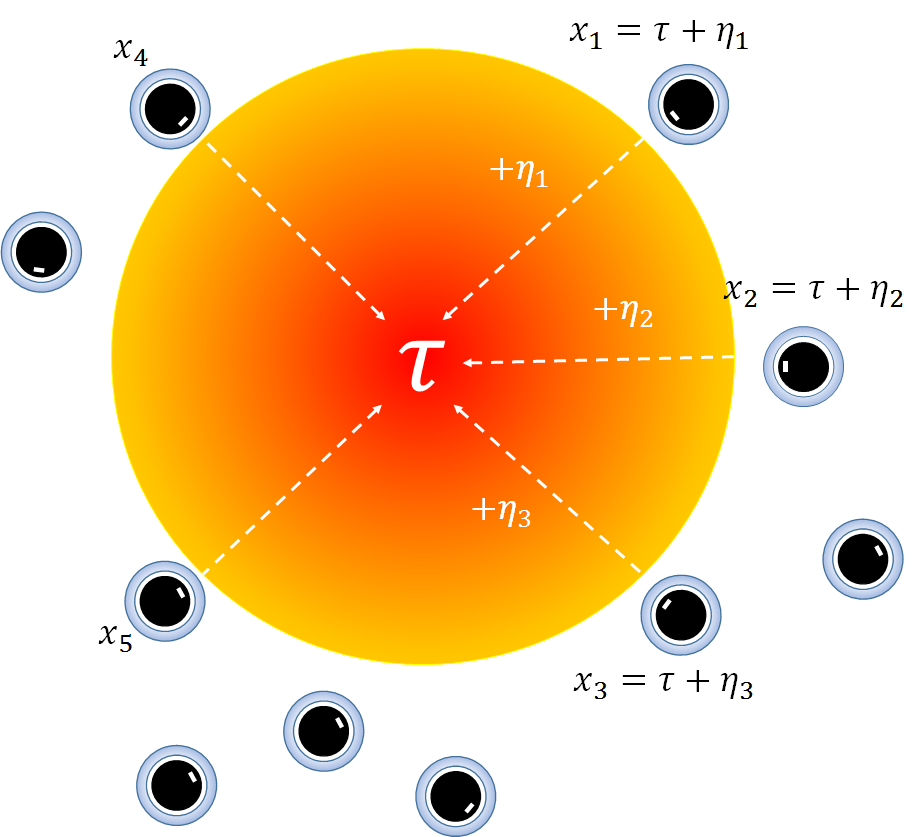
\includegraphics[height=1.2in]{figures/firefighting.png}
		\centering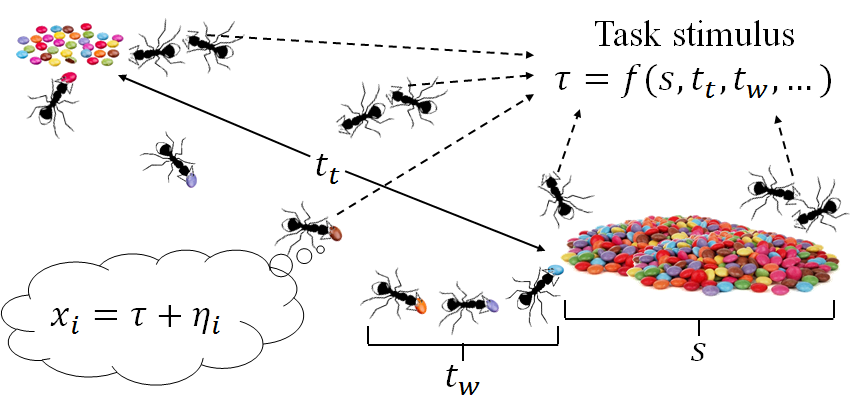
\includegraphics[height=1.1in]{figures/foraging.png}
	\centering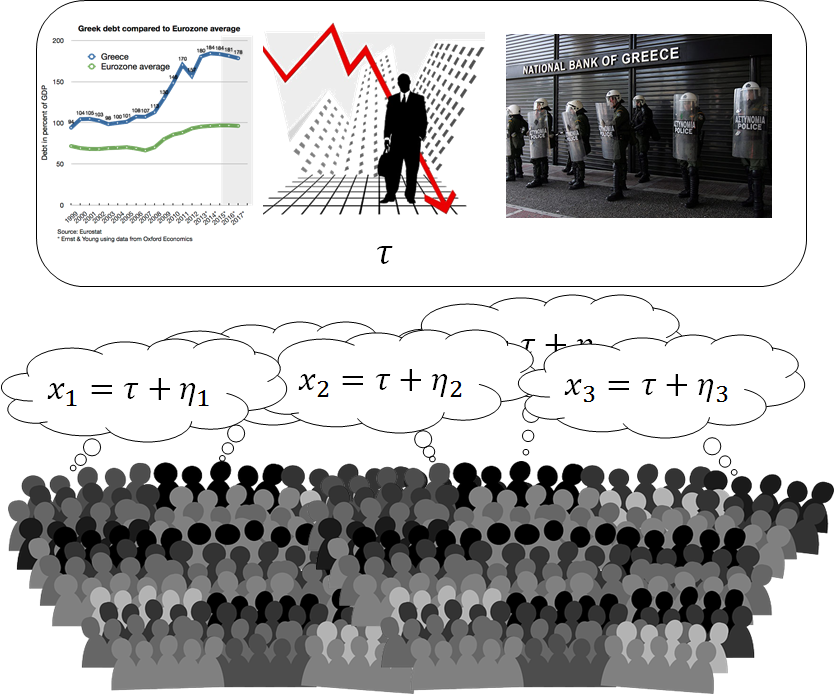
\includegraphics[height=1.2in]
{figures/bankrun.png}
	\centering\caption{Robotic fire fighting, ant foraging and bank run scenarios set up as a global game. Each player's imperfect estimate of the task is represented by $x_i$, a sum of the global magnitude parameter-$\tau$ and noisy sensor measurements-$\eta_i$. Whereas $\tau$ is representative of the minimum of number of agents needed to extinguish a fire when taking simultaneous action, it can also be representative for a cumulation of different observations such as during ant foraging, which depends on the food available in the nest, the distance to the source, and the size of the source, or the global economy such as prior to a bank run.}\vspace{-10px}
\end{figure}


\newpage
\begin{figure}[!ht]
	\centering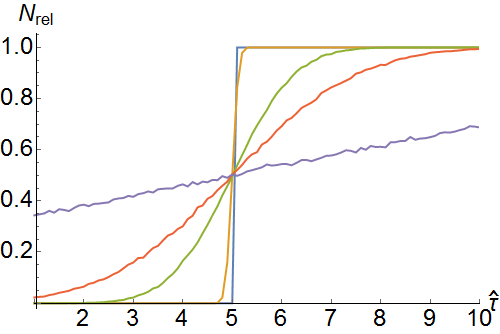
\includegraphics[width=0.3\columnwidth]{figures/thm2fig.png}
	\centering\caption{Visualization of Theorem~2 as $N_{rel}$ estimates $\Phi(\cdot)$. The plot was generated by running Eqn.~1 10,000 times for each point in $\hat{\tau} = 1$ to $10$ in increments of $0.1$. $n = 10$, $\td = 5$ and $x_i = \hat{\tau} + \eta_i$ ($\eta_i \sim\mathcal{N}(0, \sigma^2)$). Each curve in the plot is generated by sweeping $\sigma^2 = \{0, 0.1, 1, 2, 10\}$, with $\sigma^2 = 0$ being a step-function and $\sigma^2 = 10$ having the \emph{flattest} slope.}\label{fig:thm2fig}
\end{figure}
\end{document}